\begin{figure}[H]
\centering
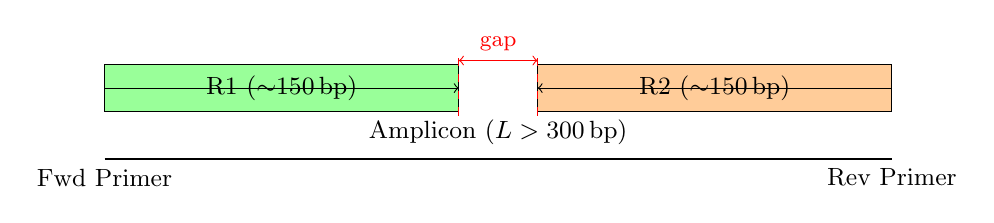
\begin{tikzpicture}[scale=1, font=\small]
  % Amplicon bar
  \draw[thick] (0,0) -- (10,0);
  \node[below] at (0,0)  {Fwd Primer};
  \node[below] at (10,0) {Rev Primer};
  \node[above] at (5, 0.05) {Amplicon ($L > 300$\,bp)};

  % R1
  \fill[green!40] (0, 0.6) rectangle (4.5, 1.2);
  \draw (0, 0.6) rectangle (4.5, 1.2);
  \node at (2.25, 0.9) {R1 ($\sim$150\,bp)};
  \draw[->] (0, 0.9) -- (4.5, 0.9);

  % R2
  \fill[orange!40] (5.5, 0.6) rectangle (10, 1.2);
  \draw (5.5, 0.6) rectangle (10, 1.2);
  \node at (7.75, 0.9) {R2 ($\sim$150\,bp)};
  \draw[<-] (5.5, 0.9) -- (10, 0.9);

  % Gap
  \draw[dashed, red] (4.5, 0.55) -- (4.5, 1.3);
  \draw[dashed, red] (5.5, 0.55) -- (5.5, 1.3);
  \draw[<->, red] (4.5, 1.25) -- (5.5, 1.25)
      node[midway, above, red, font=\footnotesize] {gap};
\end{tikzpicture}
\caption{For amplicons longer than twice the read length ($>$300\,bp with 150\,bp reads),
R1 and R2 do not meet, leaving an unsequenced gap in the centre of the amplicon.}
\label{fig:read-overlap}
\end{figure}
